\documentclass[10pt, a4paper]{article}
\usepackage[francais]{babel}
\usepackage[utf8]{inputenc}
\usepackage[T1]{fontenc}
\usepackage{hyperref}
\usepackage[]{graphicx}
\usepackage{url}
\usepackage[a4paper, left=2.5cm, right=2.5cm, top=2.0cm, bottom=2.0cm, headsep=1.0cm]{geometry}
\usepackage{subfigure}
\usepackage{epstopdf}
\usepackage{rotating}
\usepackage{wrapfig}

\setcounter{totalnumber}{5}
\renewcommand{\topfraction}{0.9}
\renewcommand{\bottomfraction}{0.9}
\newcommand{\linia}{\rule{\linewidth}{0.4mm}}

\renewcommand{\floatpagefraction}{0.7}

\newtheorem{mydef}{Definition}

\author{Yann Colin \\Grzegorz Maj}
\title{Médiathèque}

\makeatletter
\def\maketitle{%
\begin{titlepage}
	\begin{center}
		\LARGE
		\textsc{Compte rendu \\ Projet Informatique}
	\end{center}

	\vspace{3cm}

	\begin{center}\leavevmode
      \hrule
    \vskip 1pt
	\linia
	\vskip 0.5cm
	\Huge \textsc{\@title}\par

	\vskip 0.5cm
      	\linia
      \vskip 1pt
      \hrule

	\vskip 2mm

	\vspace{1.5cm}
	\begin{flushright}
		\begin{minipage}{5cm}
			\textit{\normalsize Auteurs:}\\
			\Large \textit{\@author} \par
			\vskip 2pt
			\hrule
			
		\end{minipage}
	\end{flushright}
    

	\end{center}%
	\vspace*{\stretch{6}}
    \begin{center}
    10 janvier 2016
    \end{center}
\end{titlepage}
	}
\makeatother



\begin{document}
\bibliographystyle{plain}
    \maketitle
    
    \tableofcontents
    \newpage
    
    \section{Introduction}
    
    L'objectif de ce projet est de créer un programme afin informatiser le système d'information d'une
    médiathèque. Celui-ci offrira aux adhérents des nouveaux services comme par exemple de réserver,
    d'emprunter via le logiciel des ressources. Nous avons dû utilisé la programmation orientée objet avec comme langage 
    le Java.
    
     \section{La conception}
     
	     \subsection{Diagramme de classes}
		\begin{figure}[ht]
	    \centering
	    		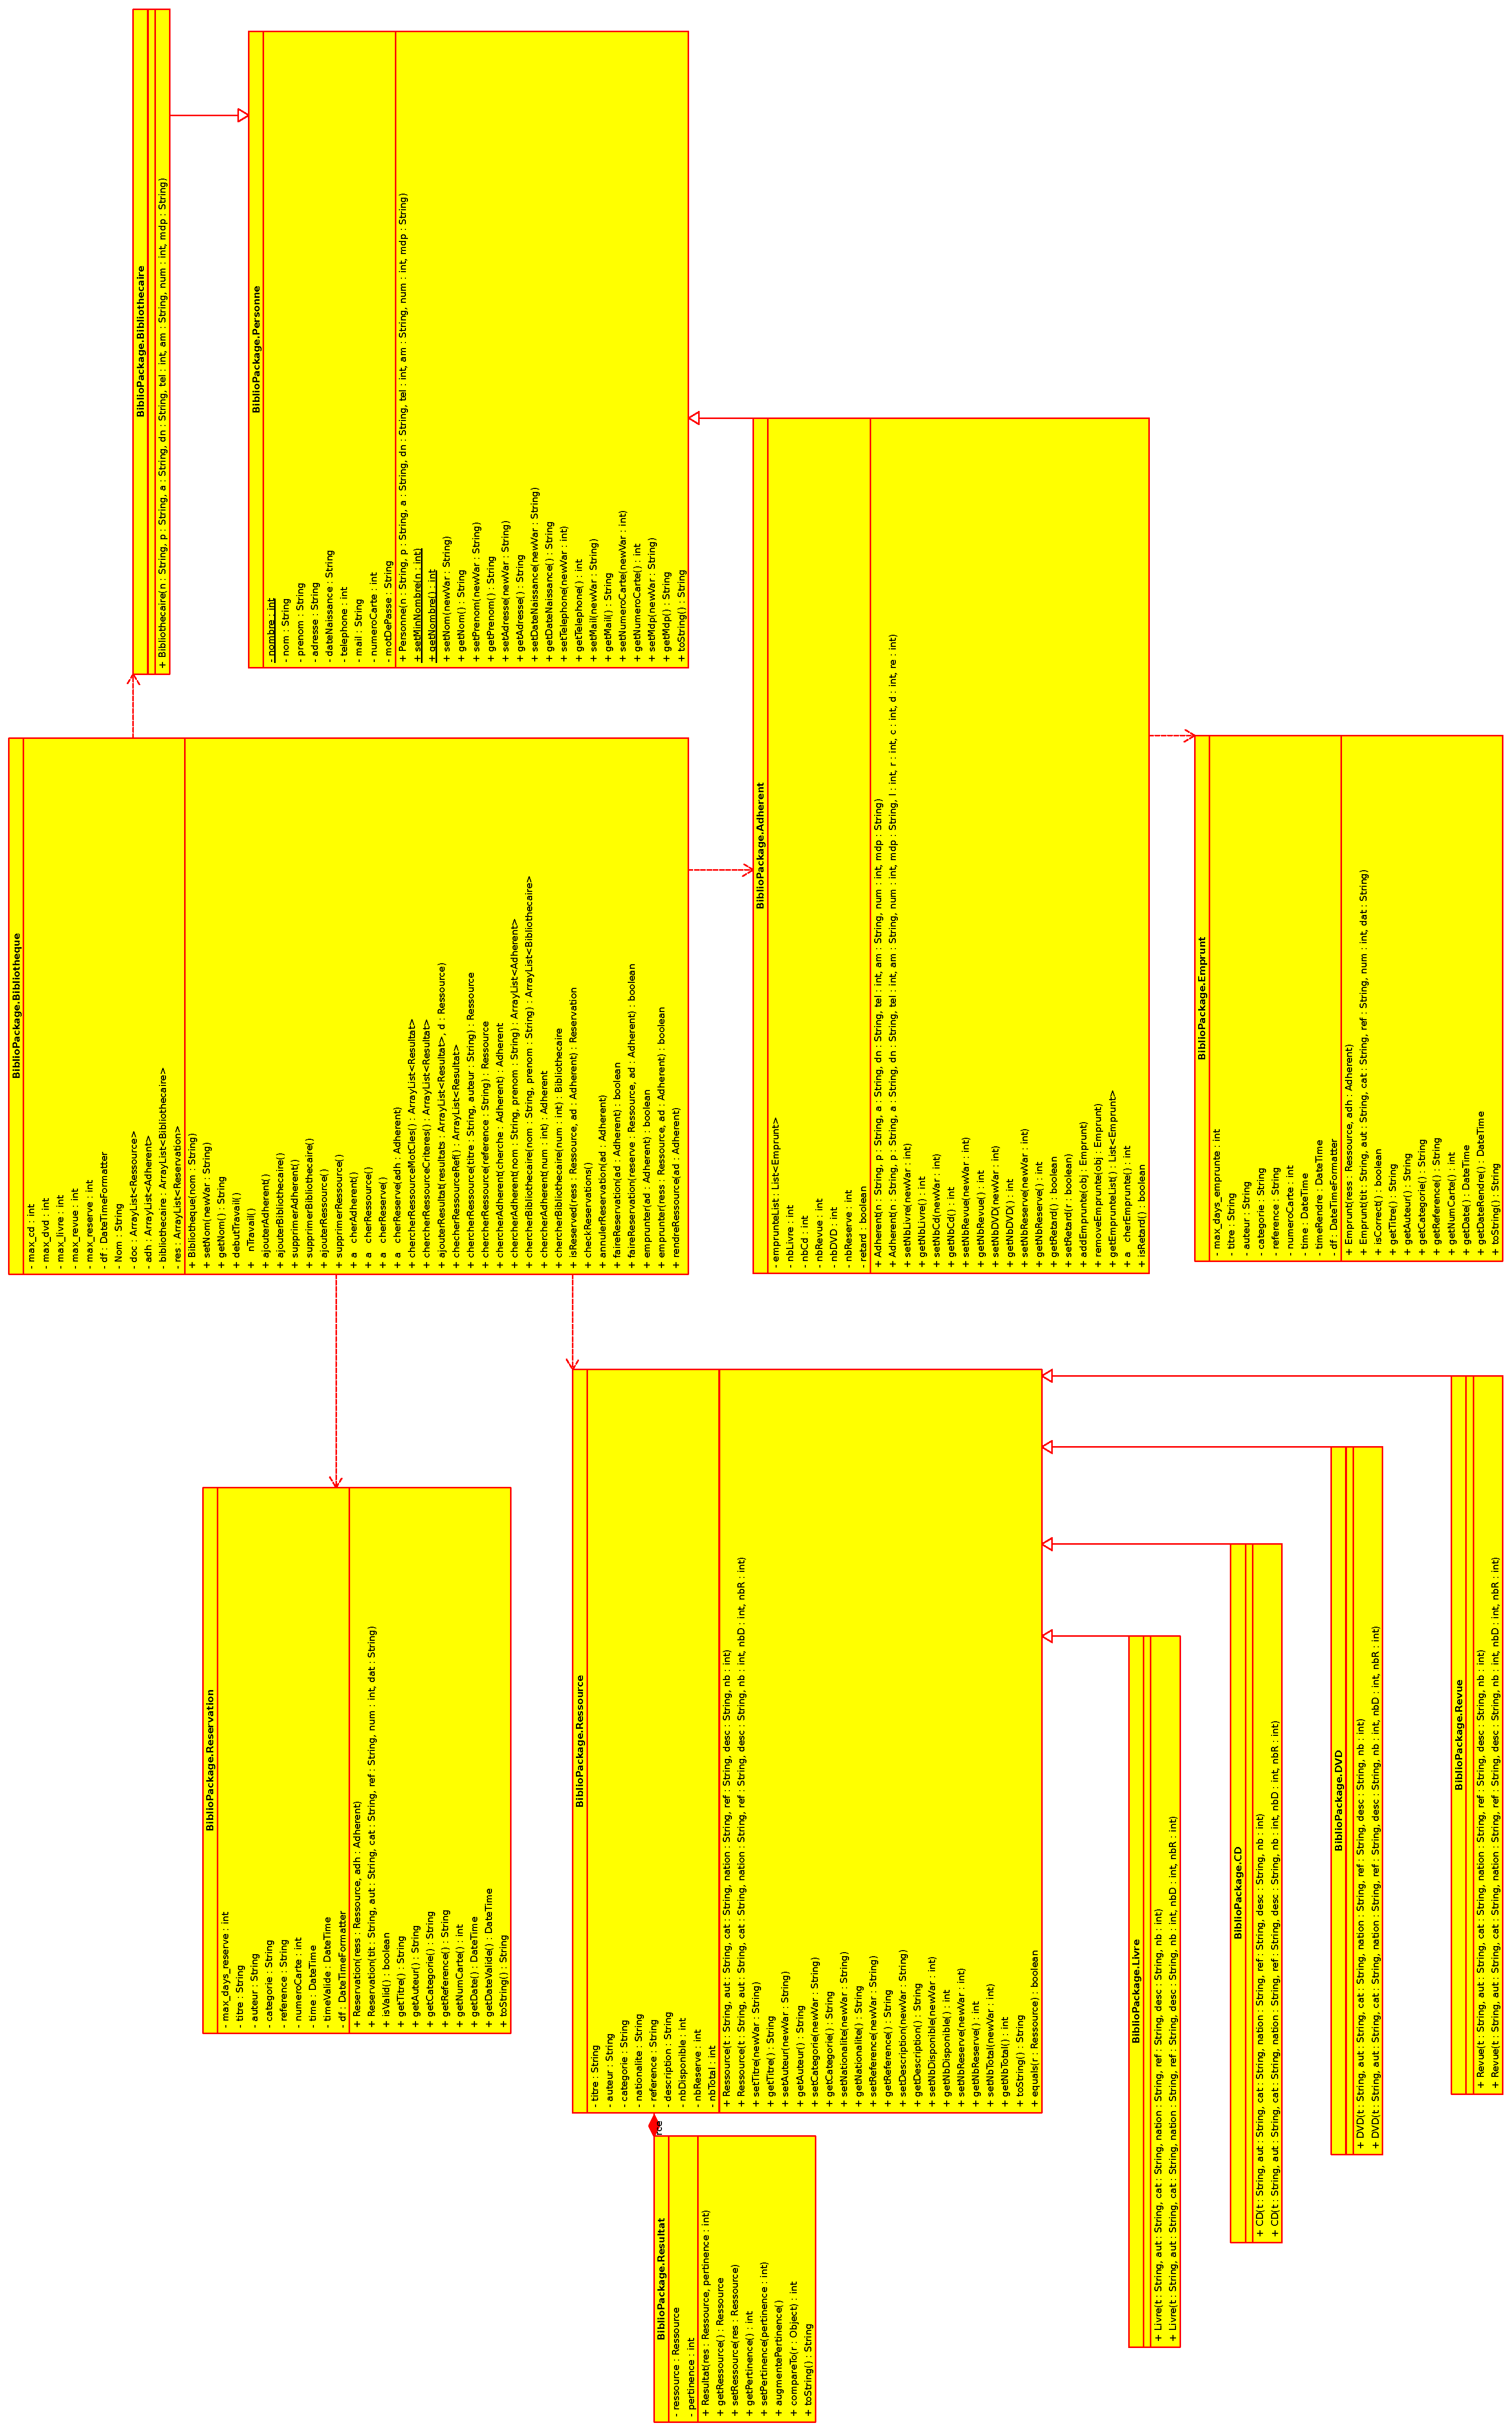
\includegraphics[width=0.7\textwidth]{graphics/class90.eps}
	    		\caption{Diagramme de classes}
	    		\label{fig:label}
	    	\end{figure}
	    	\newpage
     
    		 \subsection{Diagramme de cas d'utilisation}
    		 
    		 \begin{figure}[h]
			\begin{center}
				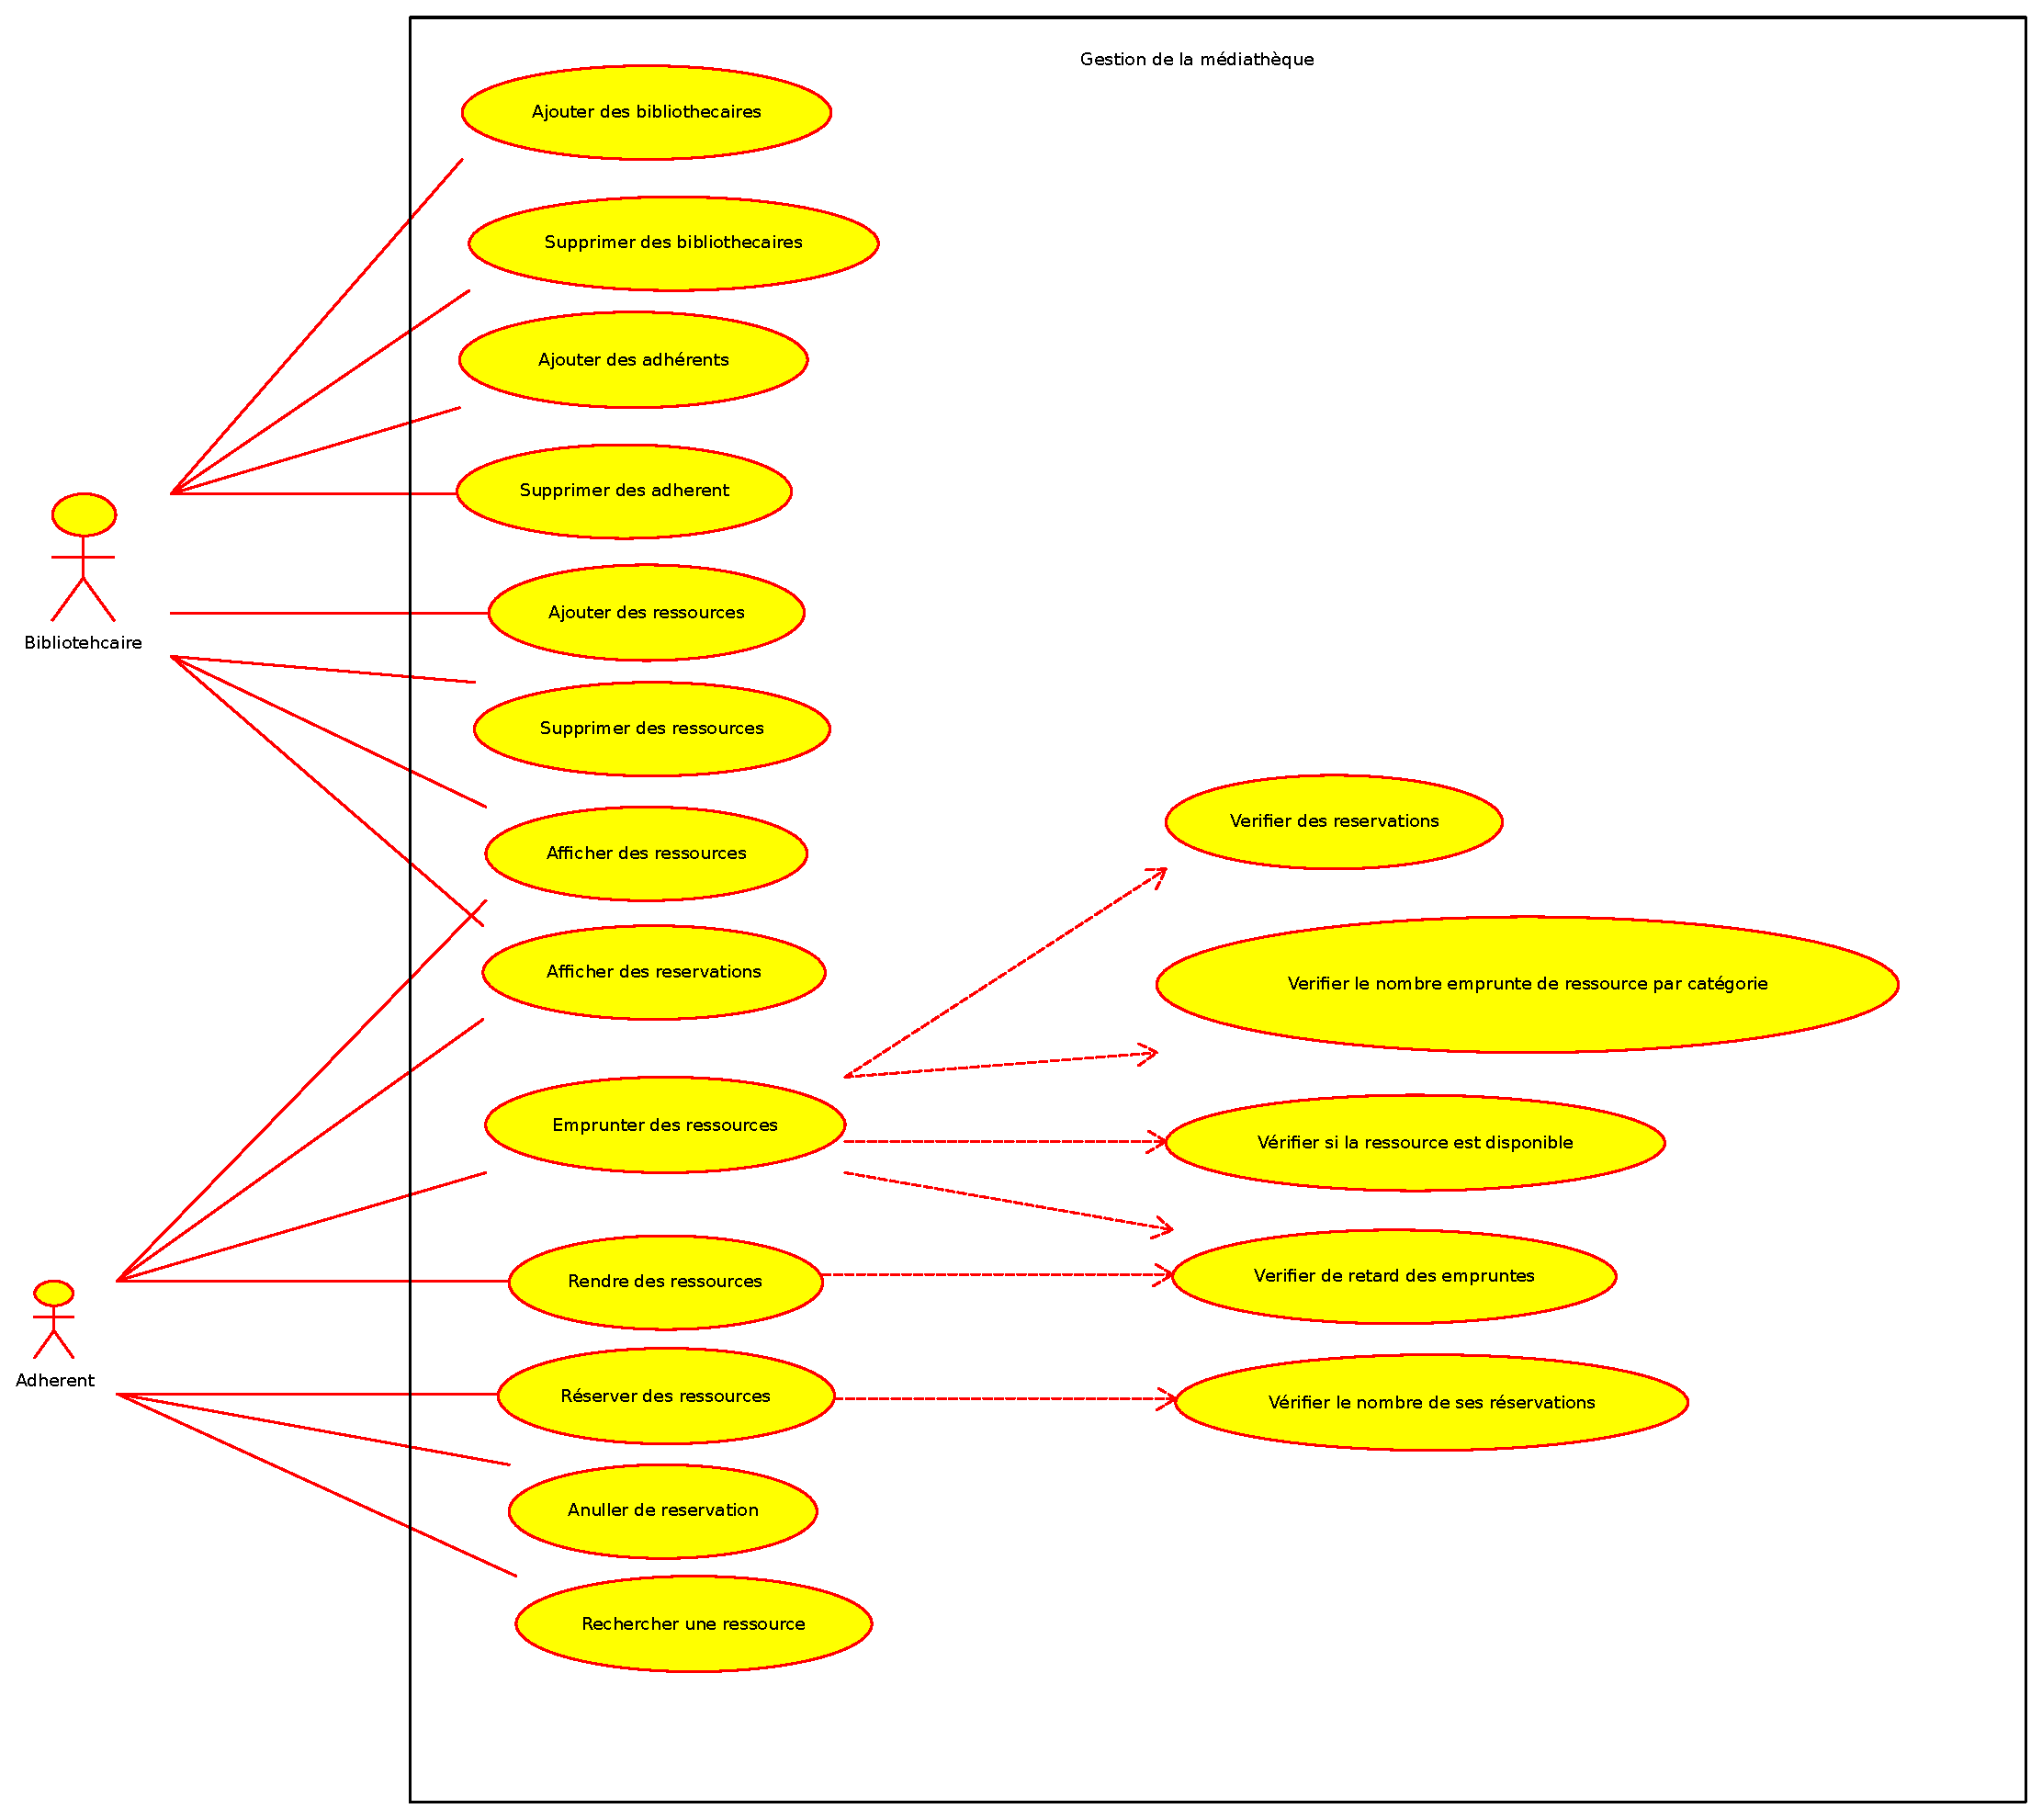
\includegraphics[width=1\textwidth]{graphics/usecasediagram.eps}
				\caption{Diagramme de cas d'utilisation.}
			\end{center}
		\end{figure}
	
	\section{Implémentation}
	Le logiciel est implémenté dans la langage Java. Pour lire les commandes de l'utilisateur on a utilisé 
	la classe \texttt{Lire}.
	
	Le projet de la médiathèque nécessite d'utiliser une base de données ou d'enregistrer les données dans des
	fichiers.
	On a considéré,comme option, l'utilisation du format XML ou du JSON. On a choisi le JSON, parce que il est plus léger et plus
	simple que le XML. Comme parser, on a choisi le JSON.simple.
	
	Pour faire les emprunts et les réservations, on a besoin d'utiliser certain format de la date. On a utilisé 
	JodaTime.
	
	\section{Les tests}
	Pendant les tests on a dû vérifier:
	\begin{enumerate}
		\item ajouter adhérent
		\item supprimer adhérent
		\item ajouter bibliothécaire
		\item supprimer bibliothécaire
		\item afficher adhérent
		\item afficher ressource
		\item ajouter ressource
		\item supprimer ressource`
		\item emprunter
		\begin{itemize}
			\item limites d'emprunt
			\item durée d'emprunt
		\end{itemize}
		\item rendre
		\item réservation
		\begin{itemize}
			\item limites de la réservation
			\item durée de  la réservation
			\item annuler une réservation
		\end{itemize}
		\item la recherche de ressources 
	\end{enumerate}
	
	
	Le processus de vérification est inclus dans le fichier ....
	
	Pour tester la date limite d'emprunt nous avons changé la durée à -1 jour afin de voir tout de suite l'effet d'un document non 
	rendu.
	
	\section{Façon de collaborer}
		\subsection{Partage du travail}
		Yann:
		\begin{itemize}
			\item diagramme de classes,
			\item diagramme de cas d'utilisation,
			\item classe Ressource + classes filles,
			\item classe Bibliothèque,
			\begin{itemize}
				\item toutes les méthodes de recherche,
				\item gestion des comptes d'adhérents et de bibliothécaires,
				\item menu pour utilisateur,
			\end{itemize}
			\item compte rendu.
			
		\end{itemize}
		
		
		Grzgorz:
		\begin{itemize}
			\item diagramme de classes,
			\item diagramme de cas d'utilisation,			
			\item classe Personne + classes filles,
			\item classe Emprunt et classe Réservation,
			\item classe Bibliothèque,
			\begin{itemize}
				\item gestion des réservations,
				\item gestion des emprunts,
				\item enregistre des données et lire de fichiers (JSON),
			\end{itemize}
			\item compte rendu.
		\end{itemize}
		
		Nous avons aussi chacun lit la partie de code, créer par l'autre, et corrigé si besoin était.
		
		\subsection{Logiciels utilisés}
		Nous avons utilisé Netbeans pour implémenter le programme, car c'est un logiciel très complet par 
		rapport a Geany.

		Pour les diagrammes de classes et d'utilisation, nous avons utilisé Umbrello qui est un logiciel 	
		très simple a utiliser.
		
		Pendant le travail, on a gardé tous les fichier sur un serveur GitHub avec utilisation du système 
		Git. Cela nous a permis de travailler en même temps, sur un même fichier sans avoir de conflits entre 
		les fichiers. Il nous permet aussi de créer différentes branches, pour différentes options et 
		ensuite d'en choisir la meilleur. Nous avons utilisé le serveur GitHub car il est gratuit, mais en 
		contrepartie tout le monde peut voir notre projet.
		
		Tout le projet est disponible sous l'adresse
		\url{https://github.com/grzegorzmaj/projetBibliotheque}.
		
		\subsection{Les problèmes}
		
		Le seul problèmes rencontré, fût de trouver une classe de date simple et stable. Il y avait un problème avec la gestion de 
		date simple et stable. Le soutien pour la date dans le langage Java n'est pas bon. La solution a était d'utilisé le JodaTime 
		qui est très connu et utilisé dans le langage Java.
		
	

\end{document}
